\subsection{بخش ب}
در این بخش فرض شده است که نیروی تراست بر اساس ربطه زیر بدست می‌آید و در هر فاز تغبرات دبی و نیروی تراست صفر است.
در ادامه نتایج آورده شده است.
\begin{figure}[H]
	\centering
	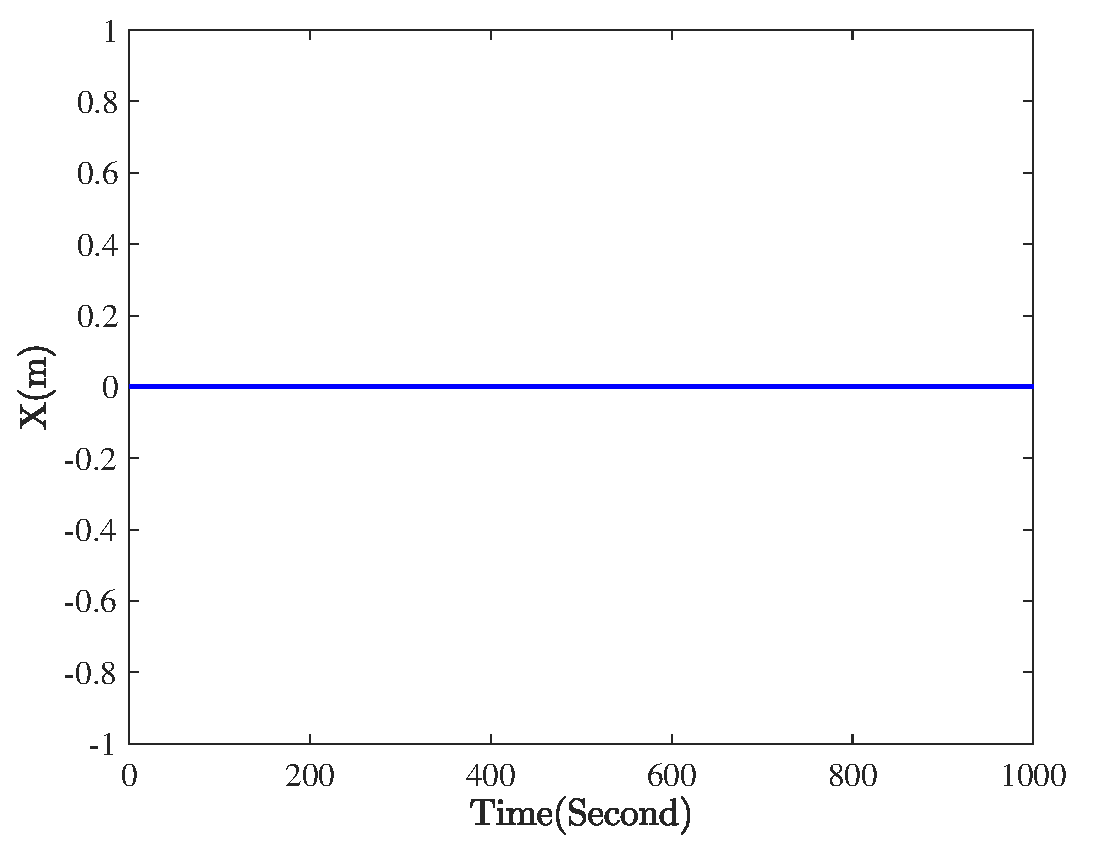
\includegraphics[width=.75\linewidth]{../Figure/Q1/b/x}
	\caption{موقعیت X پرنده تابعی از زمان}
\end{figure}
\begin{figure}[H]
	\centering
	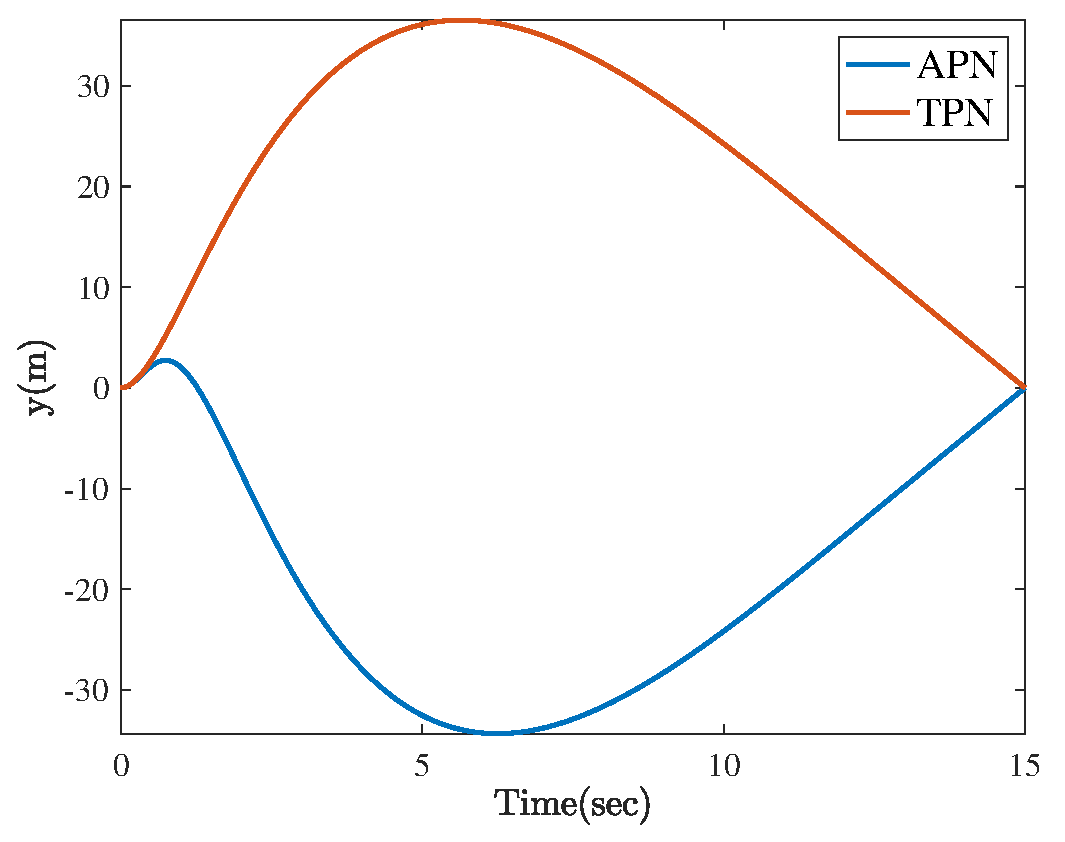
\includegraphics[width=.75\linewidth]{../Figure/Q1/b/y}
	\caption{موقعیت Y پرنده تابعی از زمان}
\end{figure}

\begin{figure}[H]
	\centering
	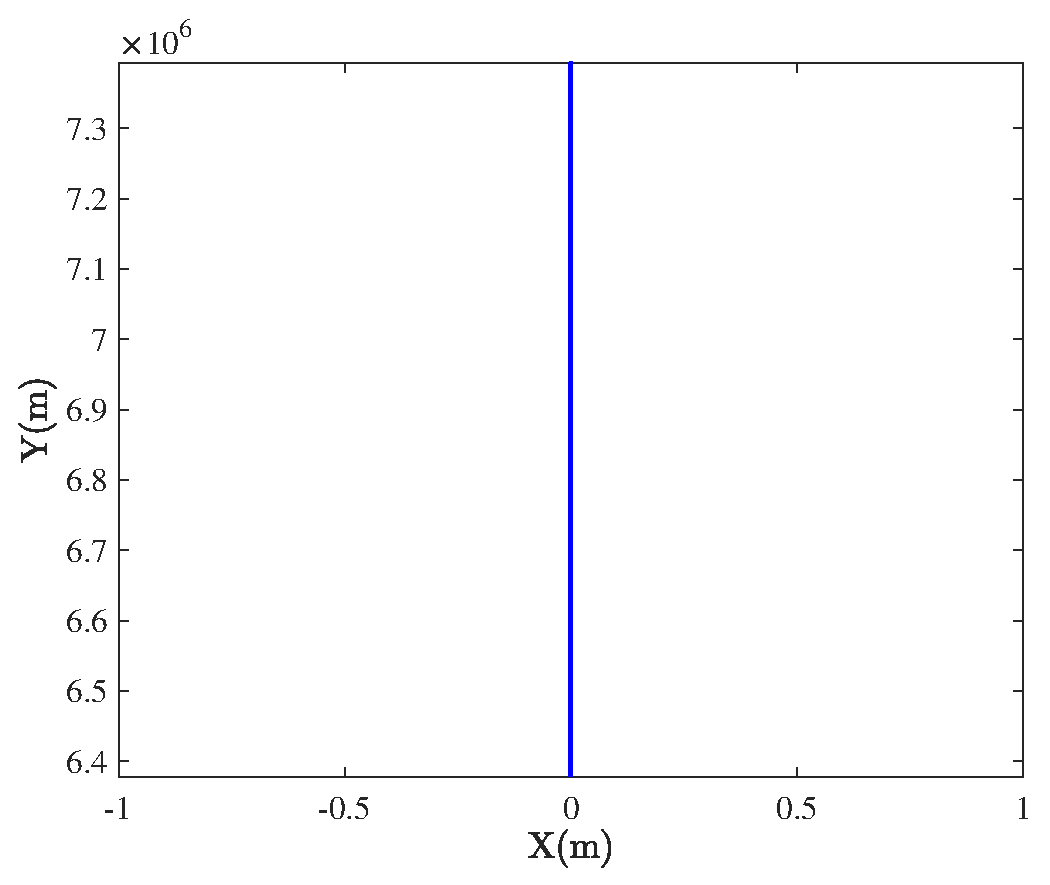
\includegraphics[width=.75\linewidth]{../Figure/Q1/b/xy}
	\caption{موقعیت پرنده در صفحه X-Y  }
\end{figure}


\begin{figure}[H]
	\centering
	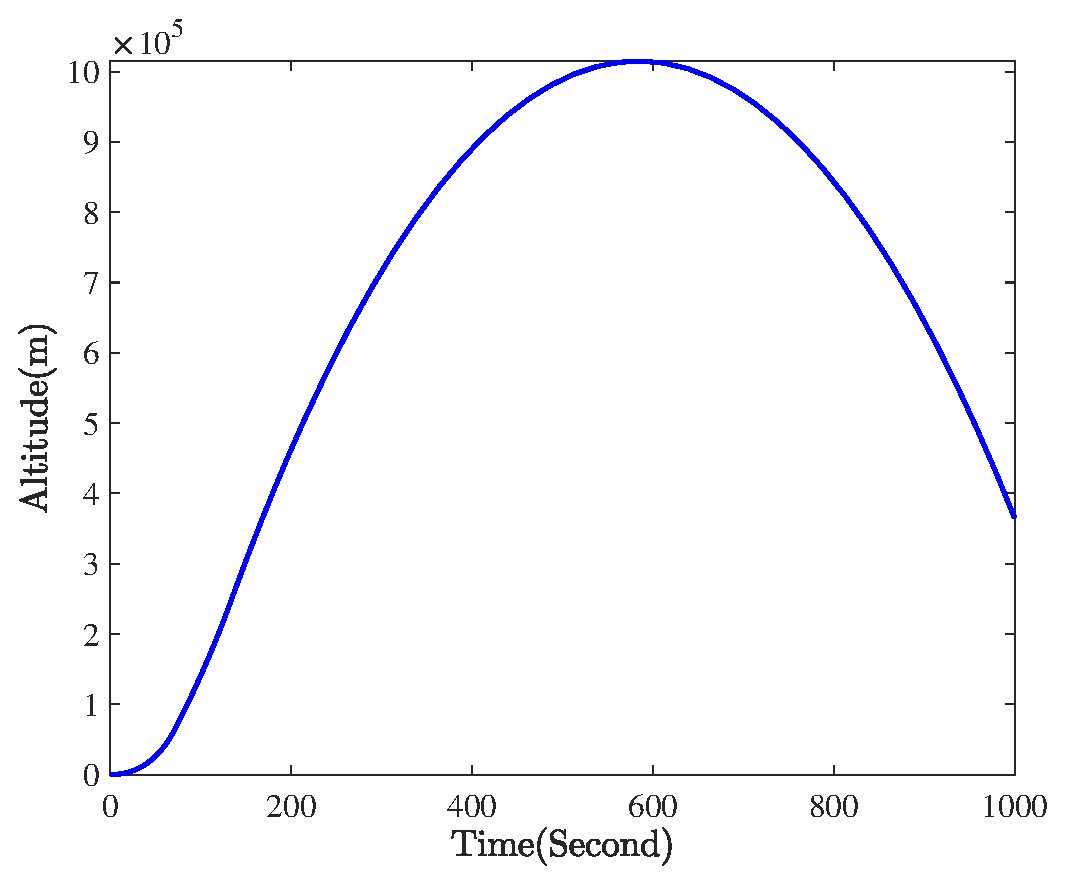
\includegraphics[width=.75\linewidth]{../Figure/Q1/b/alt}
	\caption{ارتفاع پرنده تابعی از زمان}
\end{figure}


\begin{figure}[H]
	\centering
	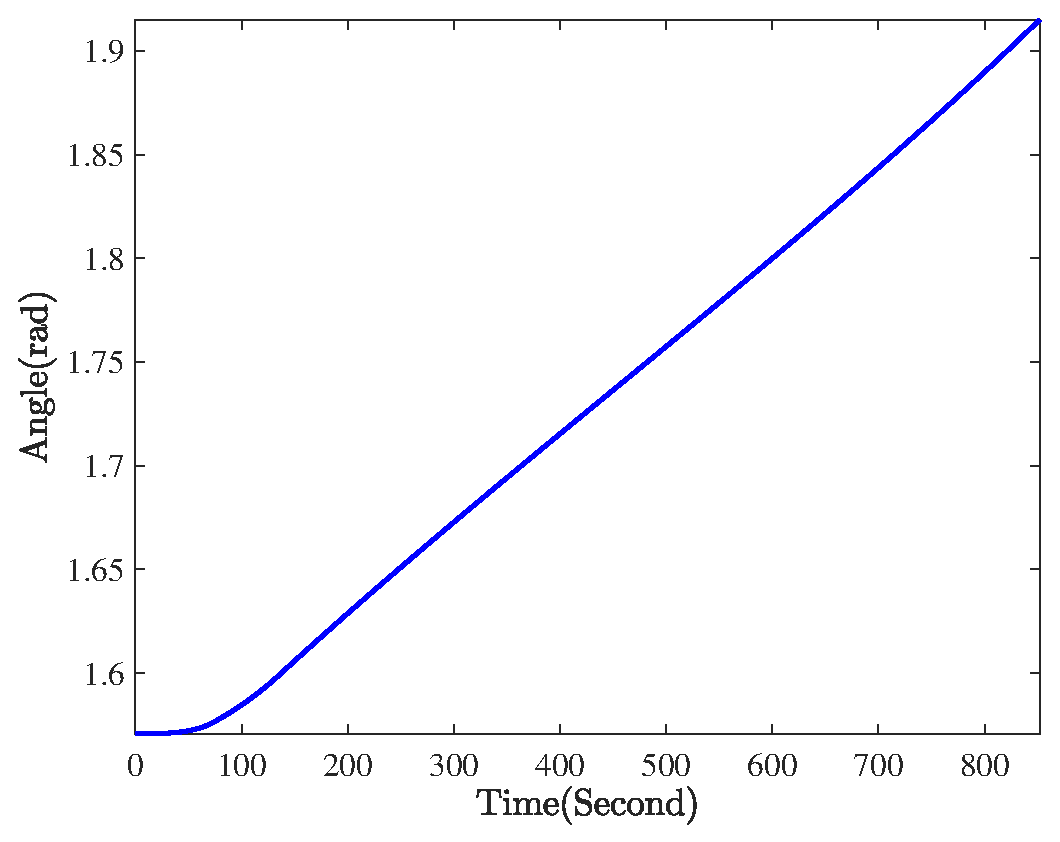
\includegraphics[width=.75\linewidth]{../Figure/Q1/b/angle}
	\caption{طول جغرافیایی پرنده تابعی از زمان}
\end{figure}


\begin{figure}[H]
	\centering
	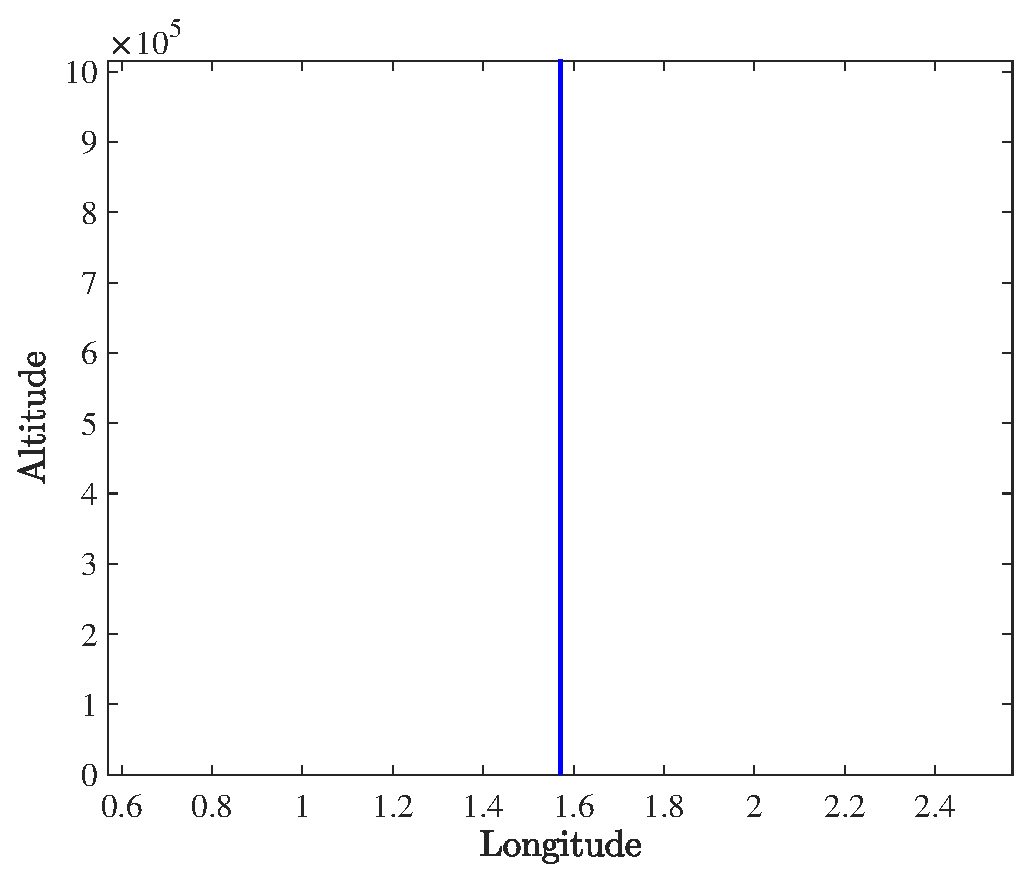
\includegraphics[width=.75\linewidth]{../Figure/Q1/b/lat_vs_alt}
	\caption{ارتفاع پرنده تابعی از طول جغرافیایی}
\end{figure}



